\documentclass[main]{subfiles}
\begin{document}
\chapter{ポールを周回しながら人が近づくと威嚇する}

これは最終課題5「警備員」の課題です。

\section{課題概要}
ロボットはポールを中心とした半径50cmの円を反時計回りに周回する。
ポールの直径は約12cm。
初期位置の制約は定められていないので、
前方もしくは左方にポールを見るような地点ならば
任意の場所からスタート可能なように設計を行った。
周回中にセンサが人に反応した場合、人とポールの間に立ち威嚇を行う。
威嚇時の動作は定められていなかったので、
ポールから2m以内の範囲で追いかける設計とした。
センサが人を捉えられなくなったり、ポールから2m以上離れてしまった場合は
再びポールの周回に戻る。

\section{解法}
物体認識やそれに伴う時間に依存しない(つまり次のサイクルに持ち越される)
同一物体判定など複雑な処理が多く、また要求される動作の種類もある程度の数が予想できたので、
現在の状態を表す変数\textit{robostate}を作成し、
ロボットの動作が以下の図のように状態遷移していくような設計にした。
\begin{figure}[H]
	\centering
	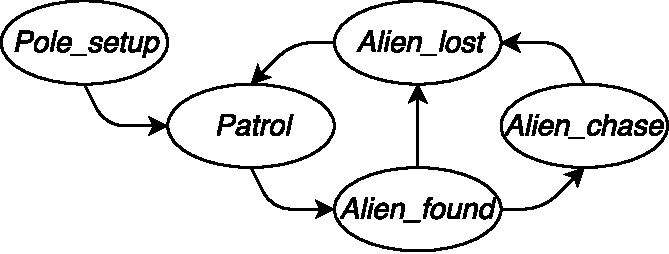
\includegraphics{img/guard_state.pdf}
	\caption{作成したプログラムの状態遷移図}
\end{figure}

\subsection{共通}
第5章と同じ方法で物体の座標を計算し、
十分近くの座標同士を同一の点群に属するものとしてオブジェクト化する。
ここで、OBJECT構造体(単なる座標データ)の配列をオブジェクトと呼称することで
若干の抽象化を図る。
同一の物体と判定を受けたものは同一の配列(OBJECT構造体の配列)に挿入され、
同一でない物体はまた別の配列に挿入される。
同一物体の座標は定数\textit{OBJBUF}を超えない範囲で配列に挿入される。

\begin{figure}[H]
	\centering
	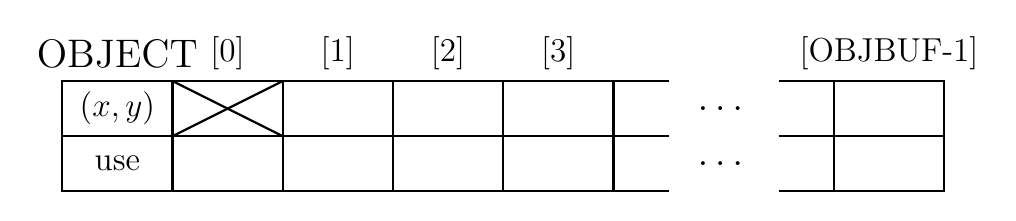
\begin{tikzpicture}[scale=0.7]
		\draw [thick] (0,0) rectangle (2,2);
		\draw [thick] (2,0) rectangle (4,2);
		\draw [thick] (4,0) rectangle (6,2);
		\draw [thick] (6,0) rectangle (8,2);
		\draw [thick] (8,0) rectangle (10,2);
		\draw [thick] (0,1) -- (11,1);
		\draw [thick] (10,0) -- (11,0);
		\draw [thick] (10,2) -- (11,2);

		\node at (1,2.5) {\Large OBJECT};
		\node at (1,1.5) {\large $(x, y)$};
		\node at (1,0.5) {\large use};
		\node at (3,2.5) {\large [0]};
		\node at (5,2.5) {\large [1]};
		\node at (7,2.5) {\large [2]};
		\node at (9,2.5) {\large [3]};

		\node at (12,1.5) {\Large \ldots };
		\node at (12,0.5) {\Large \ldots };

		\draw [thick] (14,0) rectangle (16,2);
		\draw [thick] (13,1) -- (16,1);
		\draw [thick] (13,0) -- (14,0);
		\draw [thick] (13,2) -- (14,2);

		\node at (15,2.5) {\large [OBJBUF-1]};

		\draw [thick] (2,1) -- (4,2);
		\draw [thick] (2,2) -- (4,1);
	\end{tikzpicture}
	\caption{オブジェクトの実体}
\end{figure}

今の実装では配列の最初(\textit{object[0]})は、
その配列にどこまで使用可能な値が入っているかを示す変数\textit{use}を使用するためだけに
使用しているので座標は入れない。
それ以外の\textit{use}は使用していれば1、使用していなければ0が入っている。

同一物体判定アルゴリズムの解説を行うとレポートのページ制限を軽く超えてしまうので、
詳しくは添付資料内の関数\textit{pigeonhole}を参照していただきたい。

\subsection{ポールの探索}
状態遷移図では\textit{Pole\_setup}に対応する。

ポールの探索段階では人や壁などのものが周りにないことを仮定している。
ただセンサは前方から左側のみを使用するので、
前方もしくは左方にポールを見据える形であれば右方に物体があっても動作する。

オブジェクトの中で

全状態で唯一GL座標を基準に動作する。
\subsection{パトロール}
状態遷移図では\textit{Patrol}に対応する。

\subsection{不審者発見}
状態遷移図では\textit{Alien\_found}に対応する。

\subsection{不審者追従}
状態遷移図では\textit{Alien\_chase}に対応する。

\subsection{不審者逃走}
状態遷移図では\textit{Alien\_lost}に対応する。

戻ってくる。

\section{結果}
\section{考察}

\end{document}
